\documentclass[11pt]{beamer}
\usepackage[utf8]{inputenc}
\usepackage{graphicx, epsfig}
\usepackage{amsmath,mathrsfs,amsfonts,amssymb}
%\usepackage{subfig}
\usepackage{floatflt}
\usepackage{epic,ecltree}
\usepackage{mathtext}
\usepackage{fancybox}
\usepackage{fancyhdr}
\usepackage{multirow}
\usepackage{enumerate}
\usepackage{epstopdf}
\usepackage{multicol}
\usepackage{algorithm}
\usepackage[noend]{algorithmic}
\usepackage{tikz}
\usepackage{blindtext}
\usetheme{default}%{default}%{Singapore}%{Warsaw}%{Warsaw}%{Darmstadt}
\usecolortheme{default}
\setbeamerfont{title}{size=\Huge}
\setbeamertemplate{footline}[page number]{}


\makeatletter
\newcommand\HUGE{\@setfontsize\Huge{35}{40}}
\makeatother    

\setbeamerfont{title}{size=\HUGE}
\beamertemplatenavigationsymbolsempty

% latin bold lower
\newcommand{\ba}{\mathbf{a}} 
\newcommand{\bc}{\mathbf{c}} 
\newcommand{\be}{\mathbf{e}} 
\newcommand{\bh}{\mathbf{h}} 
\newcommand{\bp}{\mathbf{p}} 
\newcommand{\bt}{\mathbf{t}} 
\newcommand{\bs}{\mathbf{s}} 
\newcommand{\bu}{\mathbf{u}} 
\newcommand{\bv}{\mathbf{v}} 
\newcommand{\bw}{\mathbf{w}} 
\newcommand{\bx}{\mathbf{x}} 
\newcommand{\by}{\mathbf{y}} 
\newcommand{\bz}{\mathbf{z}} 

% latin bold upper
\newcommand{\bA}{\mathbf{A}} 
\newcommand{\bB}{\mathbf{B}} 
\newcommand{\bC}{\mathbf{C}} 
\newcommand{\bI}{\mathbf{I}} 
\newcommand{\bL}{\mathbf{L}} 
\newcommand{\bM}{\mathbf{M}} 
\newcommand{\bQ}{\mathbf{Q}} 
\newcommand{\bT}{\mathbf{T}} 
\newcommand{\bU}{\mathbf{U}} 
\newcommand{\bV}{\mathbf{V}} 
\newcommand{\bW}{\mathbf{W}} 
\newcommand{\bX}{\mathbf{X}} 
\newcommand{\bY}{\mathbf{Y}} 
\newcommand{\bZ}{\mathbf{Z}} 

% latin cal upper
\newcommand{\cG}{\mathcal{G}} 
\newcommand{\cL}{\mathcal{L}} 
\newcommand{\cN}{\mathcal{N}} 
\newcommand{\cS}{\mathcal{S}} 
\newcommand{\cT}{\mathcal{T}} 
\newcommand{\cW}{\mathcal{W}} 
\newcommand{\cX}{\mathcal{X}} 
\newcommand{\cZ}{\mathcal{Z}} 

% latin bb upper
\newcommand{\bbE}{\mathbb{E}} 
\newcommand{\bbI}{\mathbb{I}} 
\newcommand{\bbP}{\mathbb{P}} 
\newcommand{\bbR}{\mathbb{R}} 

% greek bold lower
\newcommand{\bepsilon}{\boldsymbol{\epsilon}} 
\newcommand{\btheta}{\boldsymbol{\theta}} 
\newcommand{\blambda}{\boldsymbol{\lambda}} 
\newcommand{\bpi}{\boldsymbol{\pi}} 
\newcommand{\bmu}{\boldsymbol{\mu}} 
\newcommand{\bsigma}{\boldsymbol{\sigma}} 
\newcommand{\bphi}{\boldsymbol{\phi}} 

% greek bold upper
\newcommand{\bSigma}{\boldsymbol{\Sigma}} 

\DeclareMathOperator*{\argmin}{arg\,min}
\DeclareMathOperator*{\argmax}{arg\,max}
\newcommand{\createdgmtitle}[1]{\title[\hbox to 56mm{Mathematical Forecasting Methods \hfill\insertframenumber\,/\,\inserttotalframenumber}]
	{\vspace{1.5\cm} \\ Mathematical Forecasting Methods \\ {\Huge Лекция #1}}
	\author{}
	\institute{
	МФТИ
	} 
	\date{Осень, 2023}
}

\newcommand\myfootnote[1]{%
  \tikz[remember picture,overlay]
  \draw (current page.south west) +(1in + \oddsidemargin,0.5em)
  node[anchor=south west,inner sep=0pt]{\parbox{\textwidth}{%
      \rlap{\rule{10em}{0.4pt}}\raggedright\scriptsize \textit{#1}}};}

\newcommand\myfootnotewithlink[2]{%
  \tikz[remember picture,overlay]
  \draw (current page.south west) +(1in + \oddsidemargin,0.5em)
  node[anchor=south west,inner sep=0pt]{\parbox{\textwidth}{%
      \rlap{\rule{10em}{0.4pt}}\raggedright\scriptsize\href{#1}{\textit{#2}}}};}
\createdgmtitle{15}
\usepackage{tikz}
\usepackage{amsmath}
\usepackage[english,russian]{babel}
\usepackage[labelformat=empty]{caption}

\usepackage{graphicx,animate}
\usepackage{animate}
\usepackage{svg}
\usepackage{subcaption}

\usepackage{ stmaryrd }

\usetikzlibrary{arrows,shapes,positioning,shadows,trees}
\newcommand*{\defeq}{\stackrel{\text{def}}{=}}
\newcommand{\tensor}[1]{\underline{\textbf{#1}}}
\newcommand{\M}[1]{\textbf{#1}}
\newcommand{\norm}[1]{\lVert #1 \rVert }
%--------------------------------------------------------------------------------
\begin{document}
%--------------------------------------------------------------------------------
\begin{frame}[plain]
%\thispagestyle{empty}
\titlepage
\end{frame}
%=======
\begin{frame}{Напоминание: CP-разложение и разложение Такера}
$\tensor{X} \in \mathbb{R}^{I_1 \times I_2 \times \dots \times I_N}$ - тензор $N$-ого порядка. \\
Пусть $I = \max\{I_1, ..., I_N\}$, тогда число элементов $\tensor{X}$ есть $O(I^N)$.
\begin{itemize}
    \item Каноническое разложение: 
    $$\tensor{X} = \sum_{r=1}^R \M{b}_r^{(1)} \circ \M{b}_r^{(2)} \circ ... \circ \M{b}_r^{(N)} =  \llbracket \tensor{I}; \M{B}^{(1)}, \M{B}^{(2)}, \dots,  \M{B}^{(N)} \rrbracket$$
    Число элементов разложения: $O(NIR)$, где минимальное $R$ -- канонический ранг тензора, причем $R \leq I^{N-1}$.
    \item Разложение Такера, $\tensor{G} \in \mathbb{R}^{R_1 \times R_2 \times \dots \times R_N}$ -- центральный тензор $N$-ого порядка:
    $$ \tensor{X} = \llbracket \tensor{G}; \M{U}^{(1)}, \dots, \M{U}^{(N)} \rrbracket := \tensor{G} \times_1 \M{U}^{(1)} \times_2 \M{U}^{(2)} \times_3 \dots \times_N \M{U}^{(N)} $$
    Число элементов разложения: $O(NIR + R^N)$, где $R = \max\{R_1, ..., R_N\}$.
    
\end{itemize}
\end{frame}

%=======
\begin{frame}{Напоминание: свёртка тензоров}
\begin{itemize}
    \item (N, 1)-свёртка (contraction) тензоров $\tensor{A} \in \mathbb{R}^{I_1 \times \dots \times I_N}$ и $\tensor{B} \in \mathbb{R}^{J_1 \times \dots \times J_M}$, где обязательно $I_N = J_1$, даёт тензор 
    $\tensor{С} \in \mathbb{R}^{I_1 \times \dots \times I_{N-1} \times J_2 \times \dots \times J_M}$ с элементами:

    $$\tensor{C} = \tensor{A} \times_N^1 \tensor{B} = \tensor{A} \times^1 \tensor{B} = \tensor{A} \bullet \tensor{B}$$ 
    $$c_{i_1, ..., i_{N-1}, j_2, ..., j_M} = \sum_{i_N = 1}^{I_N} a_{i_1, ..., i_{N-1}, i_N} b_{i_N, j_2, ..., j_M}$$
\end{itemize}
Замечания:
\begin{itemize}
    \item Свёртку можно осуществлять вдоль произвольных мод исходных тензоров: $\tensor{C} = \tensor{A} \times_n^m \tensor{B}$, требование совпадения соответствующих размерностей сохраняется.
    \item Свёртку также можно осуществлять по нескольким модам тензоров-участников одновременно: операция определяется двумя упорядоченными наборами индексов мод первого и второго тензоров, с условием совпадения соответствующих размерностей в каждой паре (см. лекцию 10). 
\end{itemize}

\end{frame}
%=======
\begin{frame}{Напоминание: графическое представление тензоров}
\begin{figure}
    \centering
    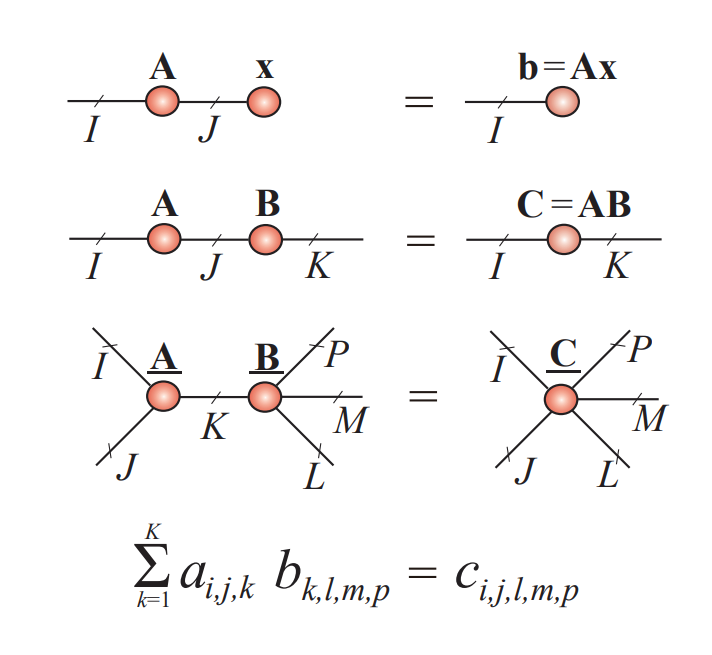
\includegraphics[width=0.8\textwidth]{lecture_10/figs/graph_repr_2.png}
\end{figure}
\end{frame}
%=======

\begin{frame}{Разложение Tensor Train}
\begin{itemize}
\item Тензор $\tensor{X} \in \mathbb{R}^{I_1 \times ...\times I_N}$ представляется в виде последовательных свёрток тензоров:
$$ \tensor{X} = \tensor{G}^{(1)} \times^1 \tensor{G}^{(2)} \times^1 \dots \times^1 \tensor{G}^{(N)} = \tensor{G}^{(1)} \bullet \tensor{G}^{(2)} \bullet \dots \bullet \tensor{G}^{(N)}
$$
\item $\tensor{G}^{(n)} \in \mathbb{R}^{R_{n-1}\times I_n \times R_n}, \ n \in \overline{1,N}$ -- тензоры 3-его порядка.
\item Полагаем $R_0 = R_N = 1$.
\item При этом говорят, что тензор $\tensor{X}$ представлен в виде TT-разложения с TT-рангом $\M{r}_{TT} = \{R_1, \dots, R_{N-1} \}$.
\end{itemize}
\vspace{0.2cm}
\begin{figure}
    \centering
    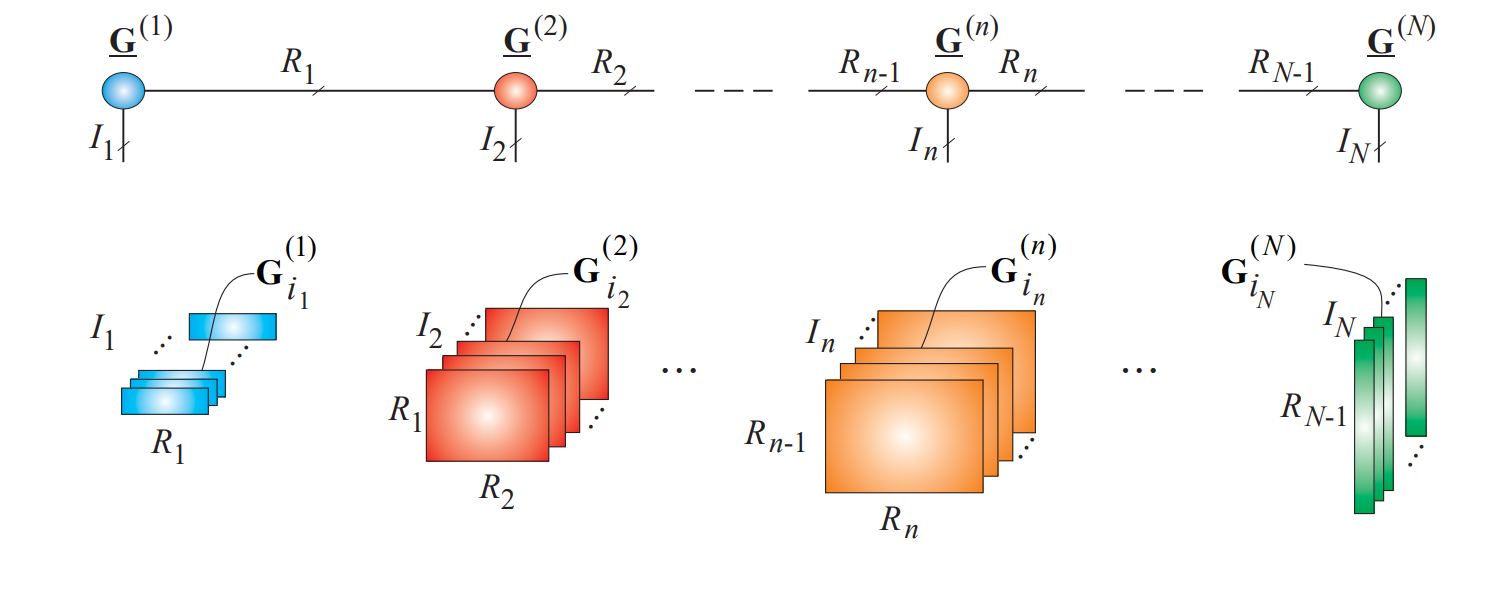
\includegraphics[width=0.9\textwidth]{lecture_15/figs/TT.png}
\end{figure}
\end{frame}
%=======
\begin{frame}{Преимущества Tensor Train}
\begin{itemize}
    \item Число элементов разложения: $O(NIR^2)$, где $R = \max\{R_1, ..., R_{N-1}\}$.
    \item Удобство применения операций для тензоров в ТТ-формате, например, сложение:
    $$
        \begin{aligned}
            &\tensor{X} = \tensor{X}^{(1)} \times^1 \tensor{X}^{(2)} \times^1 \dots \times^1 \tensor{X}^{(N)} \quad \text{(TT-разложение)}\\
            &\tensor{Y} = \tensor{Y}^{(1)} \times^1 \tensor{Y}^{(2)} \times^1 \dots \times^1 \tensor{Y}^{(N)} \quad \text{(TT-разложение)}\\
            &\tensor{Z} = \tensor{X} + \tensor{Y} = \tensor{Z}^{(1)} \times^1 \tensor{Z}^{(2)} \times^1 \dots \times^1 \tensor{Z}^{(N)}\\
            &\M{r}_{TT}(\tensor{Z}) = \M{r}_{TT}(\tensor{X}) + \M{r}_{TT}(\tensor{Y}), \quad  \tensor{Z}^{(n)} \in \mathbb{R}^{(R^{X}_{n-1} + R^{Y}_{n-1}) \times I_n \times (R^{X}_{n} + R^{Y}_{n})}\\
            &\tensor{Z}_{:, i_n, :}^{(n)} = 
            \begin{bmatrix}
            \tensor{X}_{:, i_n, :}^{(n)} & \M{0} \\
            \M{0} & \tensor{Y}_{:, i_n, :}^{(n)} 
            \end{bmatrix}, \ n \in \overline{2, N-1}\\
            &\tensor{Z}_{:, i_n, :}^{(1)} = 
            \begin{bmatrix}
            \tensor{X}_{:, i_n, :}^{(1)} & \tensor{Y}_{:, i_n, :}^{(1)} 
            \end{bmatrix}, 
            \quad 
            \tensor{Z}_{:, i_n, :}^{(N)} = 
            \begin{bmatrix}
            \tensor{X}_{:, i_n, :}^{(N)}  \\
            \tensor{Y}_{:, i_n, :}^{(N)} 
            \end{bmatrix}
        \end{aligned}
    $$
    % $$ \tensor{X} = \tensor{X}^{(1)} \times^1 \tensor{X}^{(2)} \times^1 \dots \times^1 \tensor{X}^{(N)} \quad \text{(TT-разложение)} $$
    % $$ \tensor{Y} = \tensor{Y}^{(1)} \times^1 \tensor{Y}^{(2)} \times^1 \dots \times^1 \tensor{Y}^{(N)} \quad \text{(TT-разложение)}$$
    % $$ \tensor{Z} = \tensor{X} + \tensor{Y} = \tensor{Z}^{(1)} \times^1 \tensor{Z}^{(2)} \times^1 \dots \times^1 \tensor{Z}^{(N)}$$
    % $$ \M{r}_{TT}(\tensor{Z}) = \M{r}_{TT}(\tensor{X}) + \M{r}_{TT}(\tensor{Y}), \quad  \tensor{Z}^{(n)} \in \mathbb{R}^{(R^{X}_{n-1} + R^{Y}_{n-1}) \times I_n \times (R^{X}_{n} + R^{Y}_{n})}$$
    % $$ \tensor{Z}_{:, i_n, :}^{(n)} = 
    % \begin{bmatrix}
    % \tensor{X}_{:, i_n, :}^{(n)} & \M{0} \\
    % \M{0} & \tensor{Y}_{:, i_n, :}^{(n)} 
    % \end{bmatrix}, \ n \in \overline{2, N-1} $$

    % $$ \tensor{Z}_{:, i_n, :}^{(1)} = 
    % \begin{bmatrix}
    % \tensor{X}_{:, i_n, :}^{(1)} & \tensor{Y}_{:, i_n, :}^{(1)} 
    % \end{bmatrix}, 
    % \quad 
    % \tensor{Z}_{:, i_n, :}^{(N)} = 
    % \begin{bmatrix}
    % \tensor{X}_{:, i_n, :}^{(N)}  \\
    % \tensor{Y}_{:, i_n, :}^{(N)} 
    % \end{bmatrix} $$
\end{itemize}

\end{frame}
%=======
\begin{frame}{Другие операции в ТТ-формате}
\begin{figure}
    \centering
    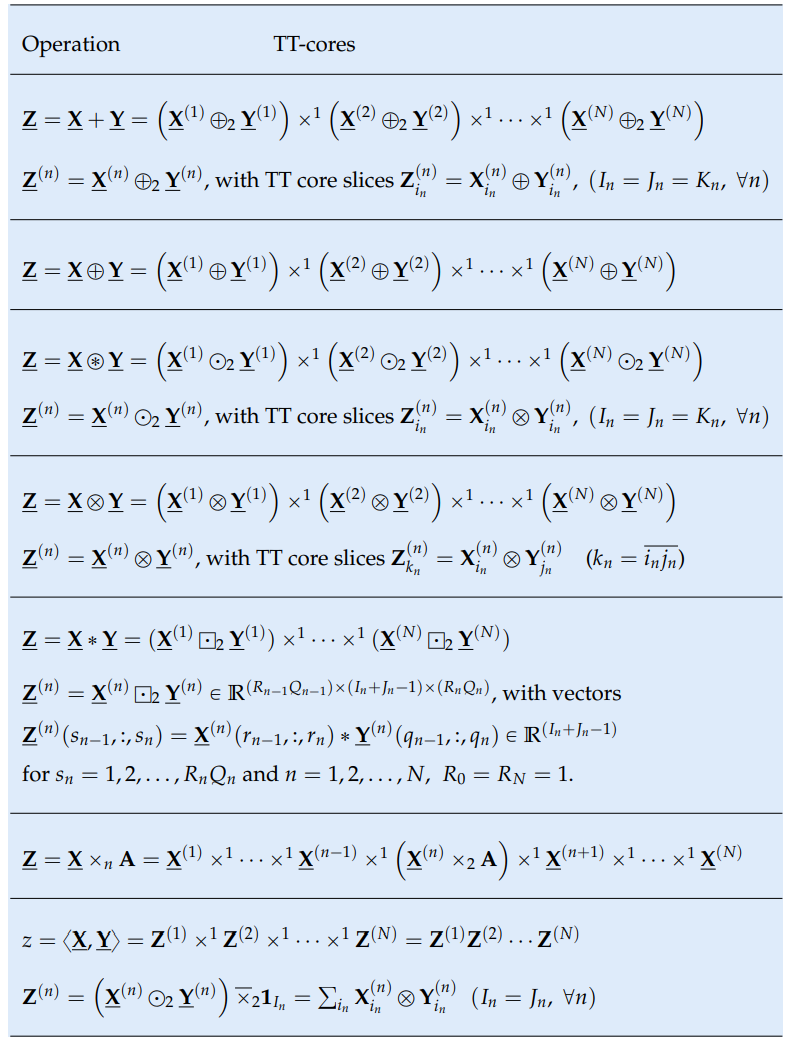
\includegraphics[width=0.7\textwidth]{lecture_15/figs/TT_operation.png}
\end{figure}
\end{frame}


%=======
\begin{frame}{Алгоритм TT-SVD Decomposition}
\begin{figure}
    \centering
    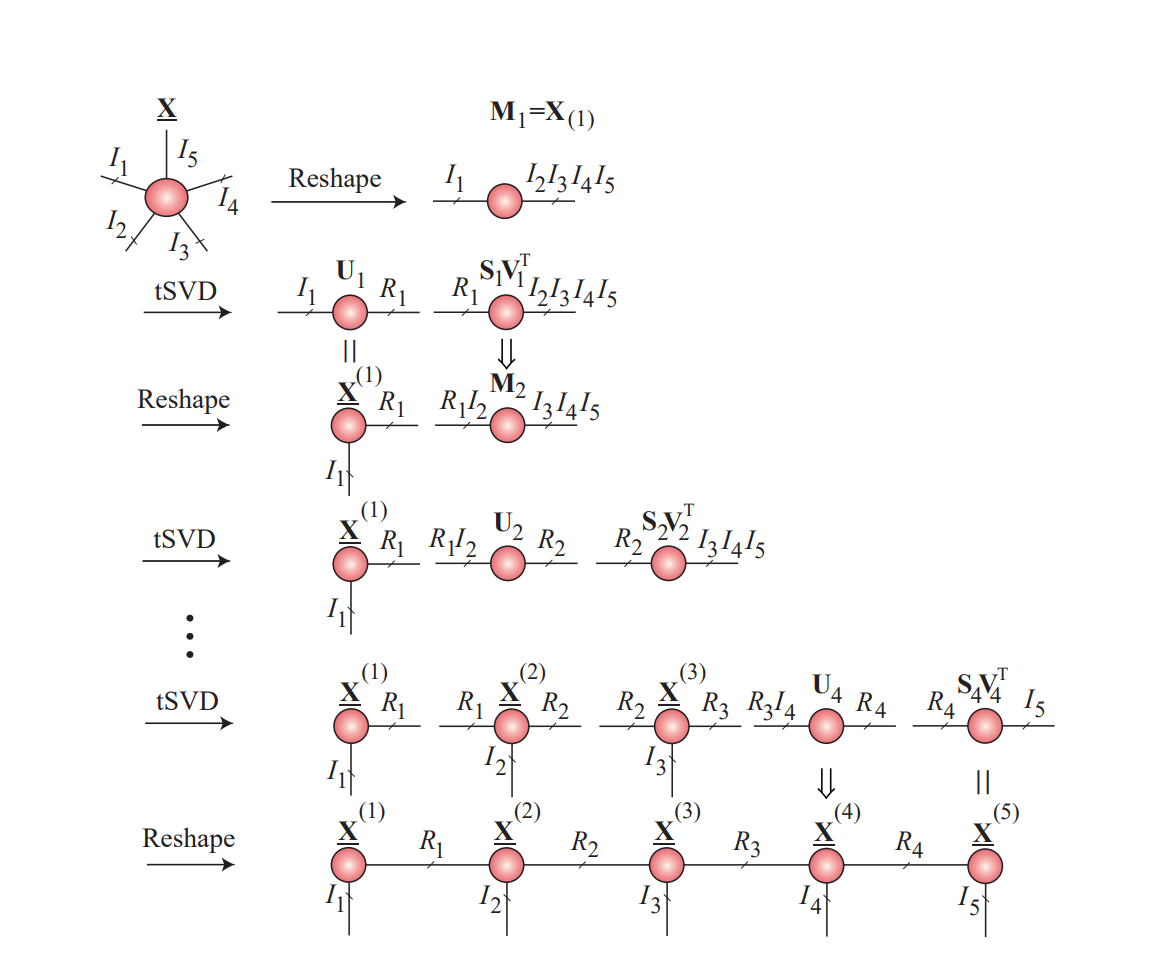
\includegraphics[width=0.9\textwidth]{lecture_15/figs/TT_algo.png}
\end{figure}
% \myfootnotewithlink{link}{сredit: text}
\end{frame}

%=======
\begin{frame}{Алгоритм TT-SVD Decomposition}

\textbf{Input:} тензор $\tensor{X} \in \mathbb{R}^{I_1 \times \dots \times I_N}$ и ошибка аппроксимации $\varepsilon$.  \\
\textbf{Output:} Приближенное представление тензора в формате ТТ $\{ \tensor{G}^{(n)} \}$, такое что $\norm{\tensor{X} - \hat{\tensor{X}}}_F \leq \varepsilon$.

\begin{enumerate}
    \item $\M{M}_1 = \tensor{X}_{(1)}$ --- развертка по 1-ой моде и $R_0 = R_N = 1$.
    \item \textbf{for} $n=1$ \textbf{to} $N-1$ \textbf{do}
    \item $\quad$ $\M{U}^{(n)}, \M{S}^{(n)}, \M{V}^{(n)} = \text{truncated\_SVD} \big(\M{M}_{n}, \frac{\varepsilon}{\sqrt{N-1}}\big)$.
    \item $\quad$ $R_n = \text{rank}(\M{U}^{(n)})$.
    \item $\quad$ $\tensor{G}^{(n)} = \text{reshape}(\M{U}^{(n)}, [ R_{n-1}, I_n, R_n])$ --- преобразование в \\ \quad \ фактор-тензор.
    \item $\quad$ $\M{M}_{n+1} = \text{reshape}(\M{S}^{(n)}\M{V}^{(n)\intercal}, [ R_n I_{n+1}, \prod_{p=n+2}^{N} I_p])$ --- \\ \quad \ преобразование в матрицу для следующей итерации.
    
    \item \textbf{end for}
    \item $\tensor{G}^{(N)} = \text{reshape}(\M{U}^{(N)}, [ R_{N-1}, I_N, R_N])$ --- преобразование в последний фактор-тензор.
    \item \textbf{return} $ \hat{\tensor{X}} = \tensor{G}^{(1)} \times^1 \dots \times^1 \tensor{G}^{(N)}$
\end{enumerate}

\end{frame}

%=======
\begin{frame}{Резюме}
\begin{itemize}
    \item Ранг канонического разложения может быть очень велик, а число элементов в разложении Такера всё ещё имеет показательную зависимость от порядка исходного тензора.
    \item Решить эту проблему можно, позволив факторам разложения быть тензорами порядка больше двух.
    \item Одно из классических разложений такого типа -- разложение Tensor Train с фактор-тензорами 3-его порядка.
    \item В Tensor-Train формате удобно осуществлять многие математические операции над тензорами.
    \item Алгоритм TT-SVD позволяет приближенно найти TT-разложение исходного тензора.
\end{itemize}
\end{frame}
\end{document} 